\documentclass[dvipdfmx]{jsarticle}
\usepackage[dvipdfmx]{graphicx}
\usepackage{subcaption}
\usepackage{here}
\usepackage{amsmath}
\usepackage{listings,jlisting}  
\begin{document}

\captionsetup{subrefformat=parens}

\title{マイクロプロセッサ レポート}
\author{高砂 爽}
\maketitle

\section{目的}
本実験ではマイクロプロセッサを用いて以下の内容を目的とする.
\begin{itemize}
    \item 2進数,10進数,16進数の相互変換と補数を用いた数値の表現
    \item アセンブリ言語を用いたプログラミング,手作業によるアセンブル
\end{itemize}

\section{実験原理・器材(KUE-CHIP2 について)}
KUE-CHIP2(Kyoto University Education-CHIP2)とは,教育用の8ビットマイクロプロセッサであり,
\begin{itemize}
    \item 京都高度技術研究所
    \item 九州大学
    \item 京都大学
    \item 立命館大学
\end{itemize}
によって開発された計算機である.
KUE-CHIP2教育用ボードには,観測や実験のために,スイッチ,表示用LED,コネクタを揃えているほか,KUE-CHIP2以外にもユーザーインターフェイスのために,多くのICを搭載している
KUE-CHIP2の特徴として,単純な命令セット・アーキテクチャを持っている.
また,動作が理解しやすいように,内部レジスタの値を観測・制御できたり,1命令・1フェーズごとに動作させたりできるという特徴がある.


\section{Problem 3.1 加算プログラムのトレース}
\subsection{実験課題(方法)}
この課題では,すでにアセンブリ言語で書かれたプログラムと機械語が与えられている.
これらを利用して,KUE-CHIP2に加算プログラムを記述し,KUE-CHIP2の基本的な使い方を学ぶ.
\subsection{与えられた式のトレース結果の表}
本節では以下の6つの式を用いて実験を行った.
\begin{table}[H]
\begin{itemize}
    \item[式(1)] $2+3$
    \item[式(2)] $126+1$
    \item[式(3)] $126+2$
    \item[式(4)] $2+(-3)$
    \item[式(5)] $(-127)+(-1)$
    \item[式(6)] $(-127)+(-2)$
\end{itemize}
\end{table}

表~\ref{table:trace_all}は,式(1)を実行した時の各トレース結果である.

また,表~\ref{table:add},表~\ref{table:adc}は式(2)から式(6)のFLAGのみの値をトレースしている.
表~\ref{table:add}では和を計算する時にADD命令を,表~\ref{table:adc}では和を計算する時にADC命令を使用している.
なお,これらの表の値はすべて16進数を用いて表現している.
\begin{table}[H]
    \caption{$2+3$を行った時の各トレース結果}
    \label{table:trace_all}
    \centering
    \begin{tabular}{|c|c|c|c|c|c|c|c|c|}
        \hline
           & PC & FLAG & ACC & IX & DBi & DBo & MAR & IR \\
           \hline\hline
           & 00 & 00 & 00 & 00 & 64 & 64 & 00 & 00 \\
           \hline
           LD ACC, [D1] P0 &$\downarrow$&&&&&&& \\
           \hline
           & 01 & 00 & 00 & 00 & 64 & 64 & 00 & 00 \\
           \hline
           LD ACC, [D1] P1 &&&&&&&& \\
           \hline
           & 01 & 00 & 00 & 00 & 64 & 64 & 00 & 64 \\
           \hline
           LD ACC, [D1] P2 &&&&&&&& \\
           \hline
           & 02 & 00 & 00 & 00 & 80 & 80 & 01 & 64 \\
           \hline
           LD ACC, [D1] P3 &&&&&&&& \\
           \hline
           & 02 & 00 & 00 & 00 & 02 & 02 & 80 & 64 \\
           \hline
           LD ACC, [D1] P4 &&&&&&&& \\
           \hline
           & 02 & 00 & 02 & 00 & 02 & 02 & 80 & 64 \\
           \hline
           ADD ACC, [D2] P0 &&&&&&&& \\
           \hline
           & 03 & 00 & 02 & 00 & B4 & B4 & 02 & 64 \\
           \hline
           ADD ACC, [D2] P1 &&&&&&&& \\
           \hline
           & 03 & 00 & 02 & 00 & B4 & B4 & 02 & B4 \\
           \hline
           ADD ACC, [D2] P2 &&&&&&&& \\
           \hline
           & 04 & 00 & 02 & 00 & 81 & 81 & 03 & B4 \\
           \hline
           ADD ACC, [D2] P3 &&&&&&&& \\
           \hline
           & 04 & 00 & 02 & 00 & 03 & 05 & 81 & B4 \\
           \hline
           ADD ACC, [D2] P4 &&&&&&&& \\
           \hline
           & 04 & 00 & 05 & 00 & 03 & 03 & 81 & B4 \\
           \hline
           ST ACC, [ANS] P0 &&&&&&&& \\
           \hline
           & 05 & 00 & 05 & 00 & 74 & 74 & 04 & B4 \\
           \hline
           ST ACC, [ANS] P1 &&&&&&&& \\
           \hline
           & 05 & 00 & 05 & 00 & 74 & 74 & 04 & 74 \\
           \hline
           ST ACC, [ANS] P2 &&&&&&&& \\
           \hline
           & 06 & 00 & 05 & 00 & 82 & 82 & 05 & 74 \\
           \hline
           ST ACC, [ANS] P3 &&&&&&&& \\
           \hline
           & 06 & 00 & 05 & 00 & 05 & 05 & 82 & 74 \\
           \hline
           ST ACC, [ANS] P4 &&&&&&&& \\
           \hline
           & 06 & 00 & 05 & 00 & 05 & 05 & 82 & 74 \\
           \hline
           HLT P0 &&&&&&&& \\
           \hline
           & 07 & 00 & 05 & 00 & 0F & 0F & 06 & 74 \\
           \hline
           HLT P1 &&&&&&&& \\
           \hline
           & 07 & 00 & 05 & 00 & 0F & 0F & 06 & 0F \\
           \hline
           HLT P2 &&&&&&&& \\
           \hline
           & 07 & 00 & 05 & 00 & 0F & 0F & 06 & 0F \\
           \hline
    \end{tabular}
\end{table}

\begin{table}[H]
    \caption{ADD命令を使用した時のFLAGトレース結果}
    \label{table:add}
    \centering
    \begin{tabular}{|c|c|c|c|c|c|}
        \hline
           式 & $126+1$ & $126+2$ & $2+(-3)$ & $(-127)+(-1)$ & $(-127)+(-2)$ \\
           \hline\hline
           計算結果 & 7F & 80 & FF & 80 & 7F \\
           \hline
           & 00 & 00 & 00 & 00 & 00 \\
           \hline
           ADC ACC, [D2] P0 & $\downarrow$ &&&&\\
           \hline
           & 00 & 00 & 00 & 00 & 00 \\
           \hline
           ADC ACC, [D2] P1 &&&&&\\
           \hline
           & 00 & 00 & 00 & 00 & 00 \\
           \hline
           ADC ACC, [D2] P2 &&&&&\\
           \hline
           & 00 & 00 & 00 & 00 & 00 \\
           \hline
           ADC ACC, [D2] P3 &&&&&\\
           \hline
           & 00 & 00 & 00 & 00 & 00 \\
           \hline
           ADC ACC, [D2] P4 &&&&&\\
           \hline
           & 00 & 06 & 02 & 02 & 04 \\
           \hline
    \end{tabular}
\end{table}

\begin{table}[H]
    \caption{ADC命令を使用した時のFLAGトレース結果}
    \label{table:adc}
    \centering
    \begin{tabular}{|c|c|c|c|c|c|}
        \hline
           式 & $126+1$ & $126+2$ & $2+(-3)$ & $(-127)+(-1)$ & $(-127)+(-2)$ \\
           \hline\hline
           計算結果 & 7F & 80 & FF & 80 & 7F \\
           \hline
           & 00 & 00 & 00 & 00 & 00 \\
           \hline
           ADC ACC, [D2] P0 & $\downarrow$ &&&&\\
           \hline
           & 00 & 00 & 00 & 00 & 00 \\
           \hline
           ADC ACC, [D2] P1 &&&&&\\
           \hline
           & 00 & 00 & 00 & 00 & 00 \\
           \hline
           ADC ACC, [D2] P2 &&&&&\\
           \hline
           & 00 & 00 & 00 & 00 & 00 \\
           \hline
           ADC ACC, [D2] P3 &&&&&\\
           \hline
           & 00 & 00 & 00 & 00 & 00 \\
           \hline
           ADC ACC, [D2] P4 &&&&&\\
           \hline
           & 00 & 06 & 02 & 0A & 0C \\
           \hline
    \end{tabular}
\end{table}
\clearpage
\subsection{フェーズ単位の実行中の各レジスタの値の変化について}
本節では式(1)を計算した時の各レジスタの値をフェーズ単位で説明する.

初めに,図~\ref{ld1}, \ref{ld2}を用いて,LD命令について記述する.
\begin{description}
    \item[P0] PCの内容"00"をMARに転送する. \\ PCが示している00番地の命令を読み出すために,MARにPCの値を転送する.MARの内容は"00"となり,PCの値はインクリメントされる.
    \vspace{2mm}
    \item[P1] 命令内容の読み出しが行われる.\\ MARの内容で指定された00番地の内容(64)が入力バスDBiを通り命令レジスタIRへ転送される.  
    \vspace{2mm}
    \item[P2] 命令デコーダIDCでIRの内容が解読される. \\ 上位4ビット"0110"はLD命令であること,下位4ビット"0100"は,対象としているレジスタがACCであること,データはプログラム領域にあることが解釈される. \\ 
    また,第二オペランドのアドレスを生成するために,2バイト目を読み出す.このため,再びMARにPCの値"01"を転送し,PCの値はインクリメントされる.
    \vspace{2mm}
    \item[P3] メモリの読み出しが行われる. \\ MARの内容で指された01番地の内容"80"が読み出され,DBi → ALU → DBoを介してMARへ転送される.
    \vspace{2mm}
    \item[P4] 第二オペランドの読み出しが行われる. \\   命令のアドレスモードはプログラム領域を指しているので,読み出されるデータのアドレスの上位ビットは"0"となる.読み出されたデータはDBi → ALU → DBoを介して,ACCに格納される.
\end{description}





\begin{figure}[H] % LD ACC
    \begin{center}
        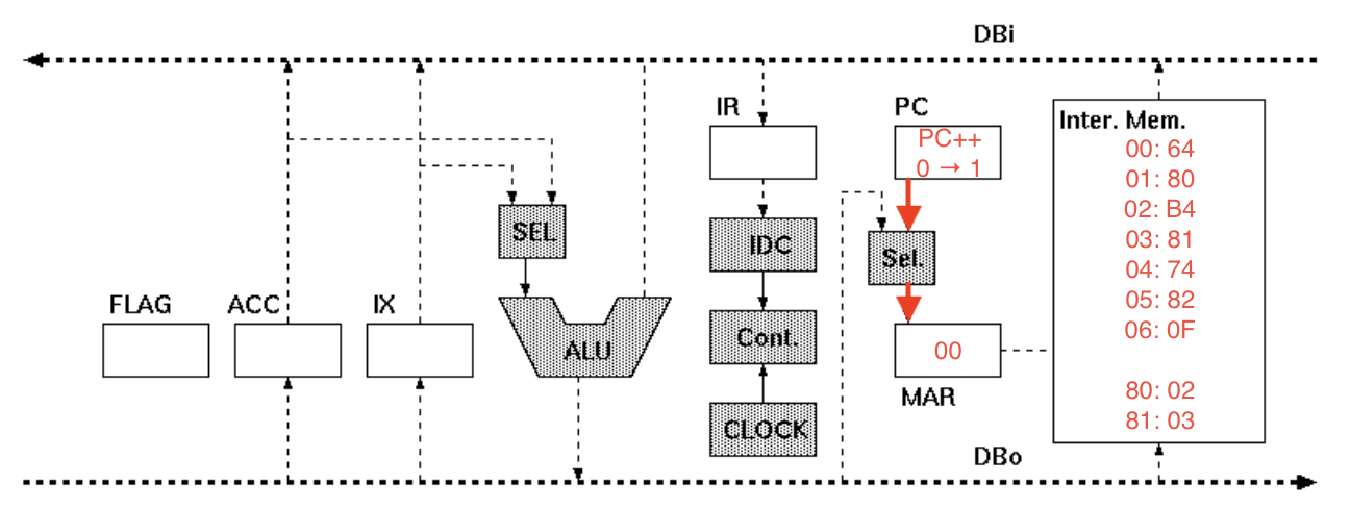
\includegraphics[scale=0.7]{img/ld0.eps}% 図を貼り込む
        \vspace{-2mm}
        \subcaption{LD ACC, [D1] P0時の値}
        \label{img:ld0}
    \vspace{1cm}
        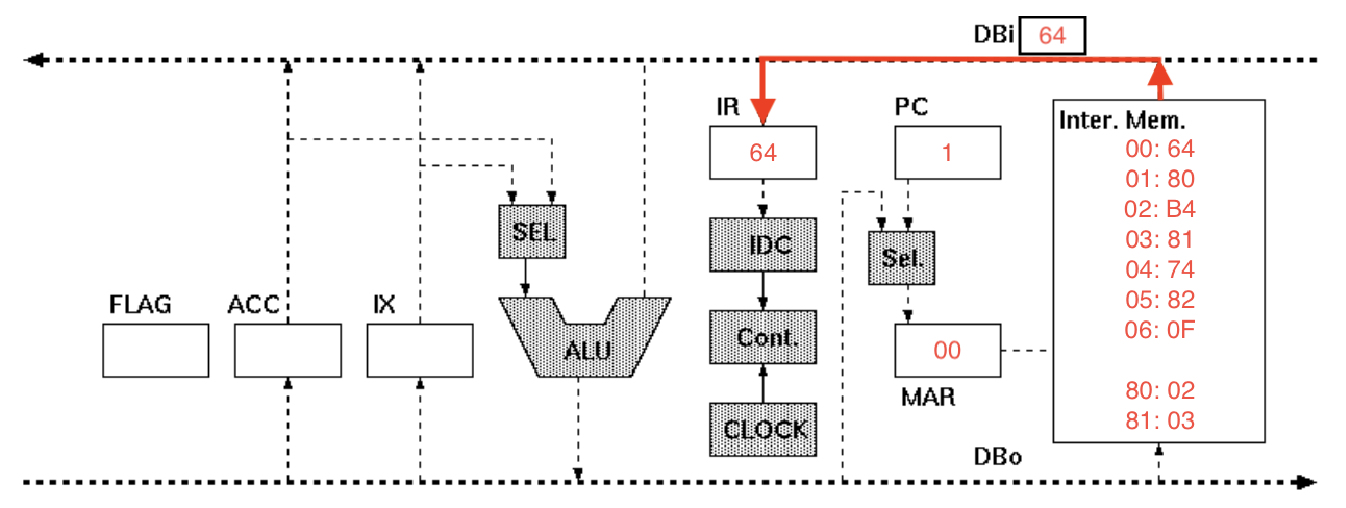
\includegraphics[scale=0.7]{img/ld1.eps}% 図を貼り込む
        \vspace{-2mm}
        \subcaption{LD ACC, [D1] P1時の値}
        \label{img:ld1}
    \vspace{1cm}
        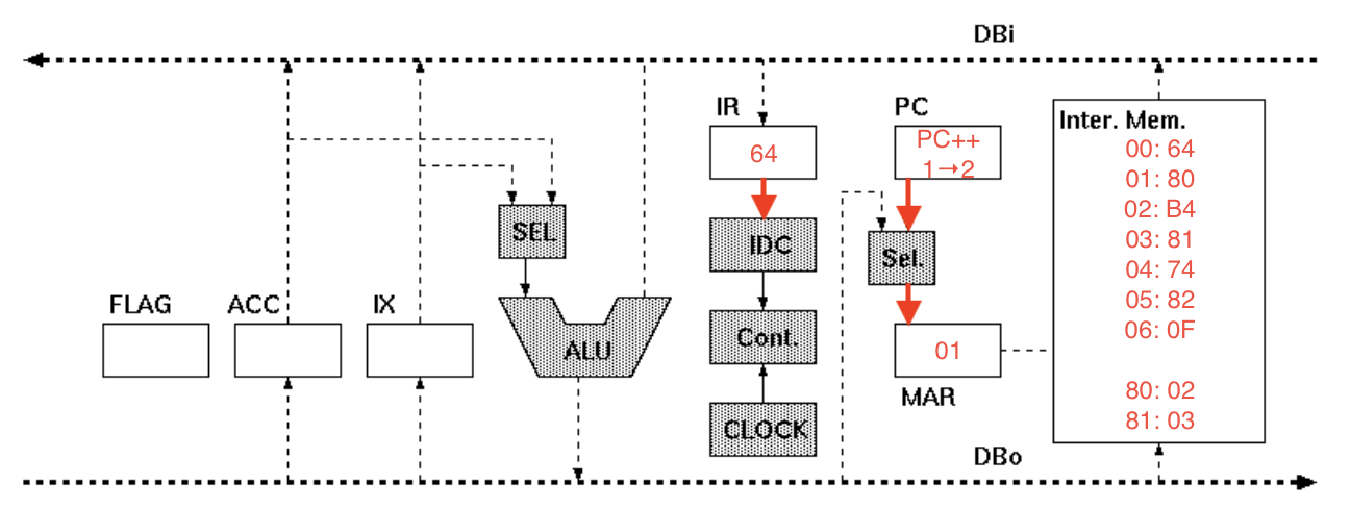
\includegraphics[scale=0.7]{img/ld2.eps}% 図を貼り込む
        \vspace{-2mm}
        \subcaption{LD ACC, [D1] P2時の値}
        \label{img:ld2}
    \vspace{1cm}
    \end{center}
    \caption{LD ACC時の各レジスタの値(1)}
    \label{ld1}
\end{figure}

\begin{figure}[H]
    \begin{center}
        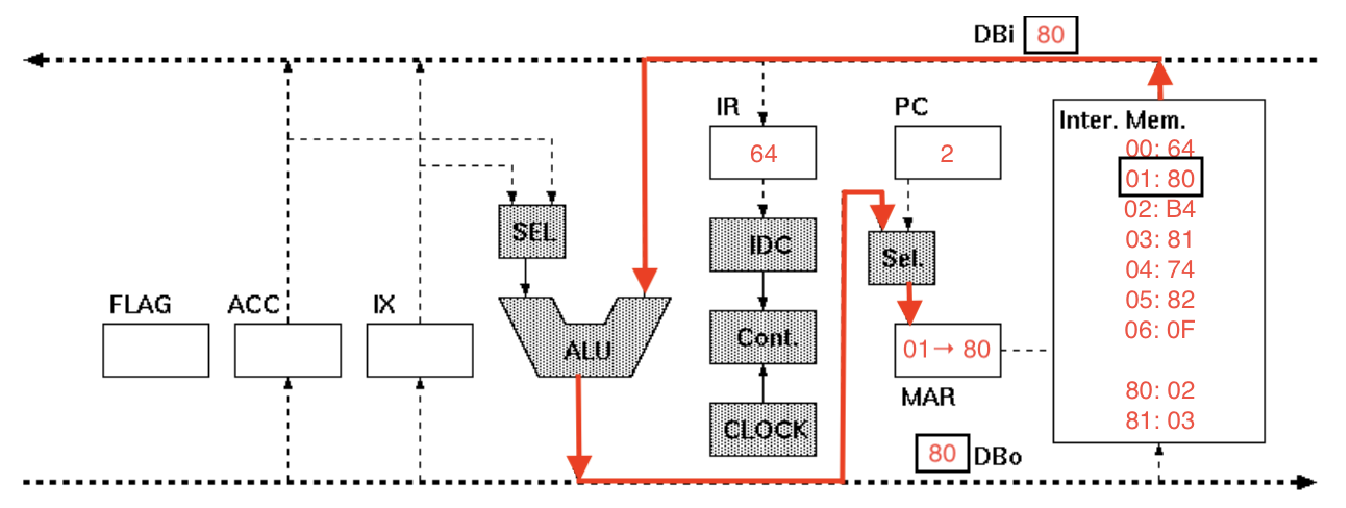
\includegraphics[scale=0.7]{img/ld3.eps}% 図を貼り込む
        \vspace{-2mm}
        \subcaption{LD ACC, [D1] P3時の値}
        \label{img:ld3}
    \vspace{1cm}
        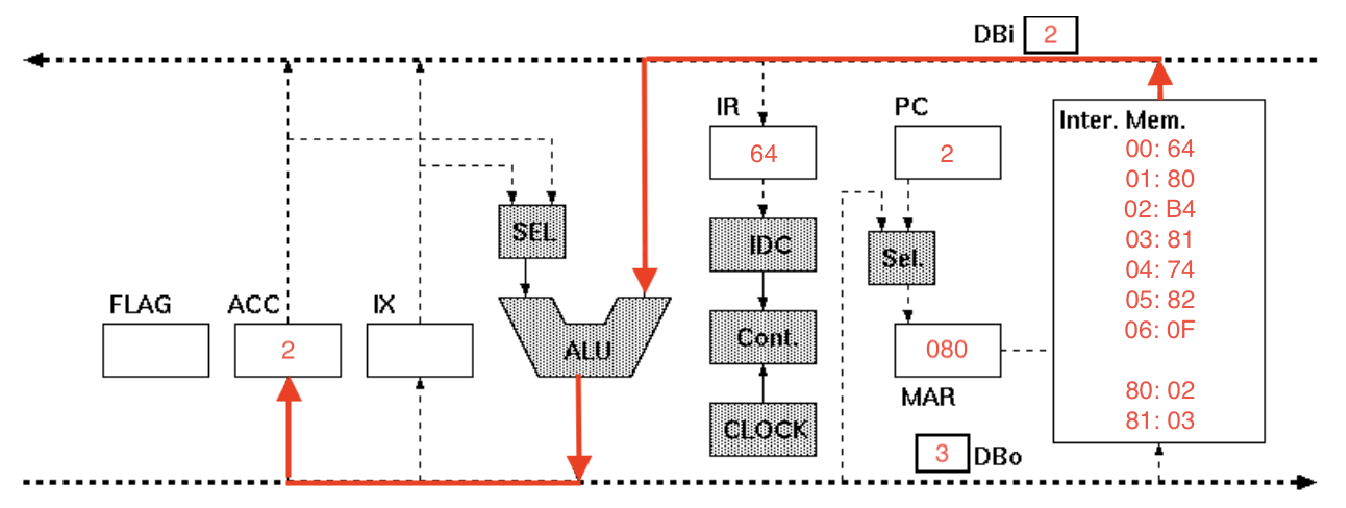
\includegraphics[scale=0.7]{img/ld4.eps}% 図を貼り込む
        \vspace{-2mm}
        \subcaption{LD ACC, [D1] P4時の値}
        \label{img:ld4}
    \end{center}
    \caption{LD ACC時の各レジスタの値(2)}
    \label{ld2}
\end{figure}

\clearpage


2つ目に,図~\ref{add}を用いて,ADD命令について記述する.
なお,P0, P1時は全ての命令において共通なので,図は省略する.
また,P2においても省略する.
\begin{description}
    \item[P0] PCの内容"02"をMARに転送する. \\ PCが示している02番地の命令を読み出すために,MARにPCの値を転送する.MARの内容は"02"となり,PCの値はインクリメントされる.
    \vspace{2mm}
    \item[P1] 命令内容の読み出しが行われる. \\ MARの内容で指定された02番地の内容(B4)が入力バスDBiを通り命令レジスタIRへ転送される.
    \vspace{2mm}
    \item[P2] 命令でコータIDCでIRの内容が解読される. \\ 上位4ビット"1011"はADD命令であること,下位4ビット"0100"は,対象としているレジスタがACCであること,データはプログラム領域にあることが解釈される. \\
    また,第二オペランドのアドレスを生成するために2バイト目を読み出す.このため,再びMARにPCの値"03"を転送し,PCの値はインクリメントされる.
    \vspace{2mm}
    \item[P3] メモリの読み出しが行われる. \\ MARの内容で示された03番地の内容"81"が読み出され,DBi → ALU → DBoを介してMARへ転送される.
    \vspace{2mm}
    \item[P4] 第二オペランドの読み出しが行われる. \\ MARの内容"81"を元に,プログラム領域にある"3"がDBiを介してALUへ転送される.また,ACCの内容"2"がALUへ転送され加算,計算結果はDBoを介してACCに格納される.
\end{description}

\begin{figure}[H] % ADD ACC
    \begin{center}
            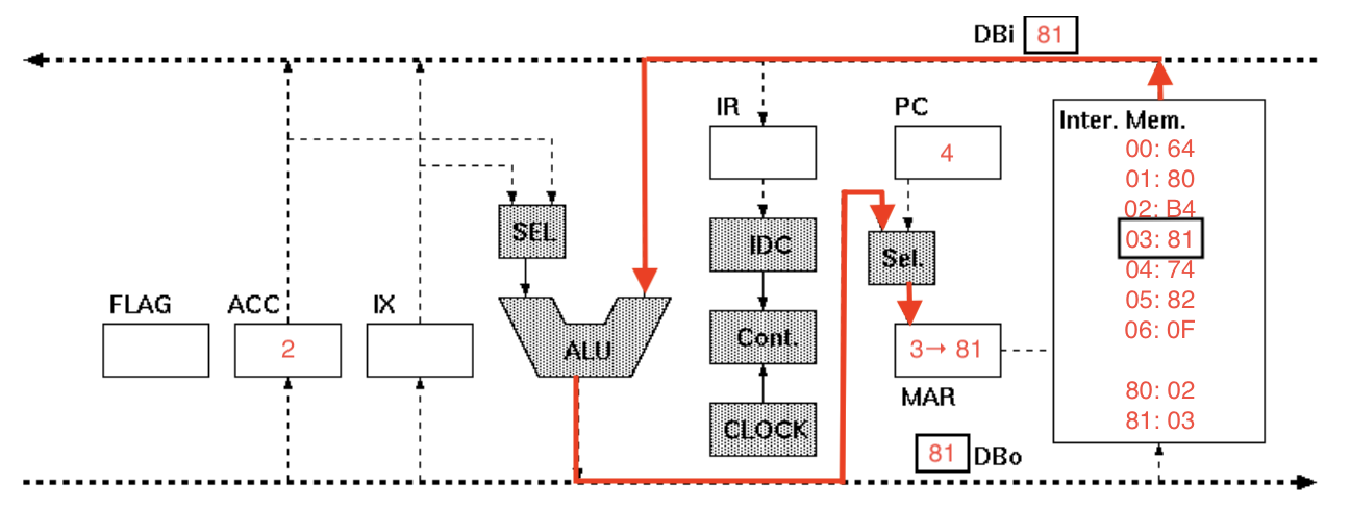
\includegraphics[scale=0.7]{img/add3.eps}% 図を貼り込む
            \vspace{-2mm}
            \subcaption{ADD ACC, [D2] P3時の値}
            \label{img:add3}
        \vspace{1cm}
            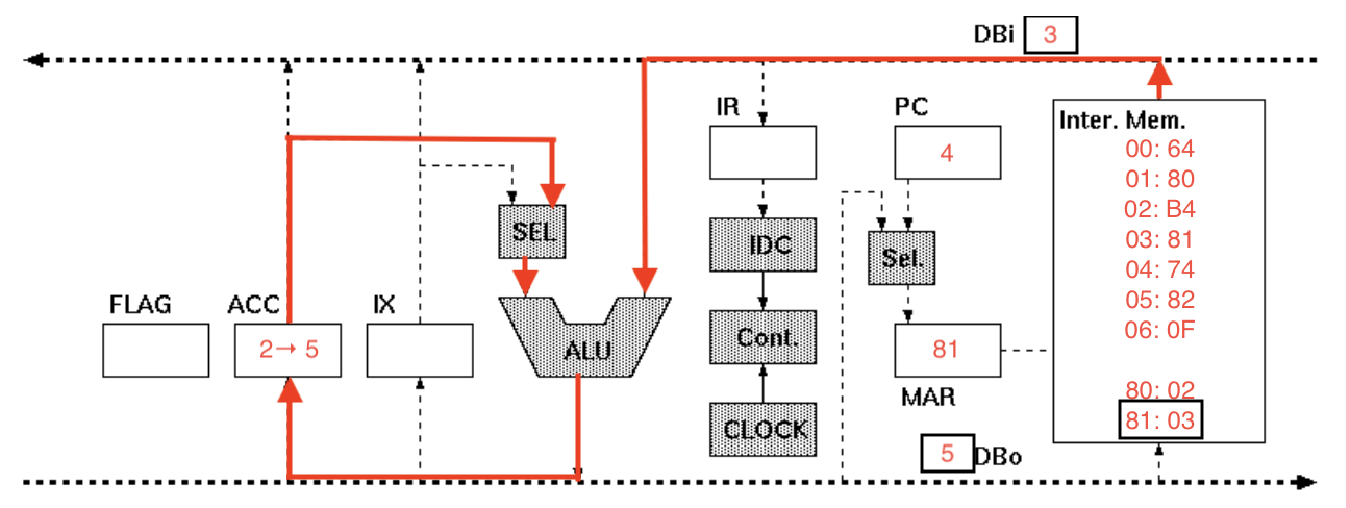
\includegraphics[scale=0.7]{img/add4.eps}% 図を貼り込む
            \vspace{-2mm}
            \subcaption{ADD ACC, [D2] P4時の値}
            \label{img:add4}
    \end{center}
    \caption{ADD ACC時の各レジスタの値}
    \label{add}
\end{figure}

\clearpage


3つ目に,図~\ref{st}を用いて,ST命令について記述する.
\begin{description}
    \item[P0] PCの内容"04"をMARに転送する. \\ PCが示している04番地の命令を読み出すために,MARにPCの値を転送する.MARの内容は"04"となり,PCの値はインクリメントされる.
    \vspace{2mm}
    \item[P1] 命令内容の読み出しが行われる. \\ MARの内容で指定された04番地の内容(74)が入力バスDBiを通り命令レジスタIRへ転送される.
    \vspace{2mm}
    \item[P2] 命令でコータIDCでIRの内容が解読される. \\ 上位4ビット"0111"はST命令であること,下位4ビット"0100"は,対象としているレジスタがACCであること,データはプログラム領域にあることが解釈される. \\
    また,第二オペランドのアドレスを生成するために2バイト目を読み出す.このため,再びMARにPCの値"05"を転送し,PCの値はインクリメントされる.
    \vspace{2mm}
    \item[P3] メモリの読み出しが行われる. \\ MARの内容で示された05番地の内容"82"が読み出され,DBi → ALU → DBoを介してMARへ転送される.
    \vspace{2mm}
    \item[P4] 第二オペランドの読み出しが行われる. \\ 命令のアドレスモードはプログラム領域を指しているので,読み出されるデータのアドレスの上位ビットは"0"となる.読み出されたデータはSEL → ALU → DBoを介して,プログラム領域に格納される.
\end{description}

\begin{figure}[H] % ST ACC
    \begin{center}
            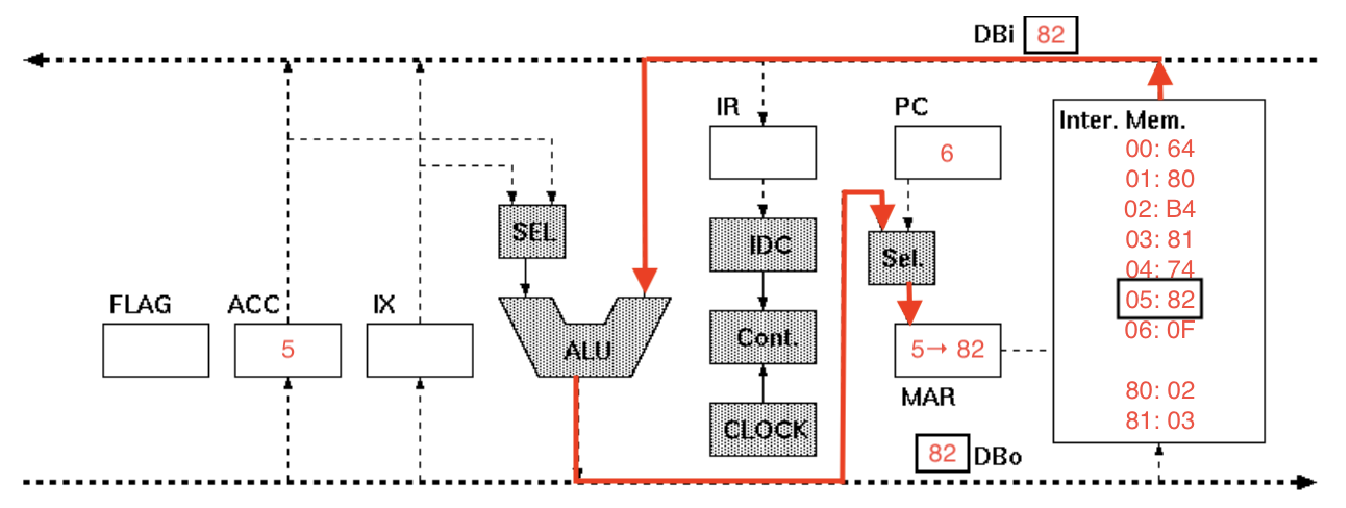
\includegraphics[scale=0.7]{img/st3.eps}% 図を貼り込む
            \vspace{-2mm}
            \subcaption{ST ACC, [ANS] P3時の値}
            \label{img:st3}
        \vspace{1cm}
            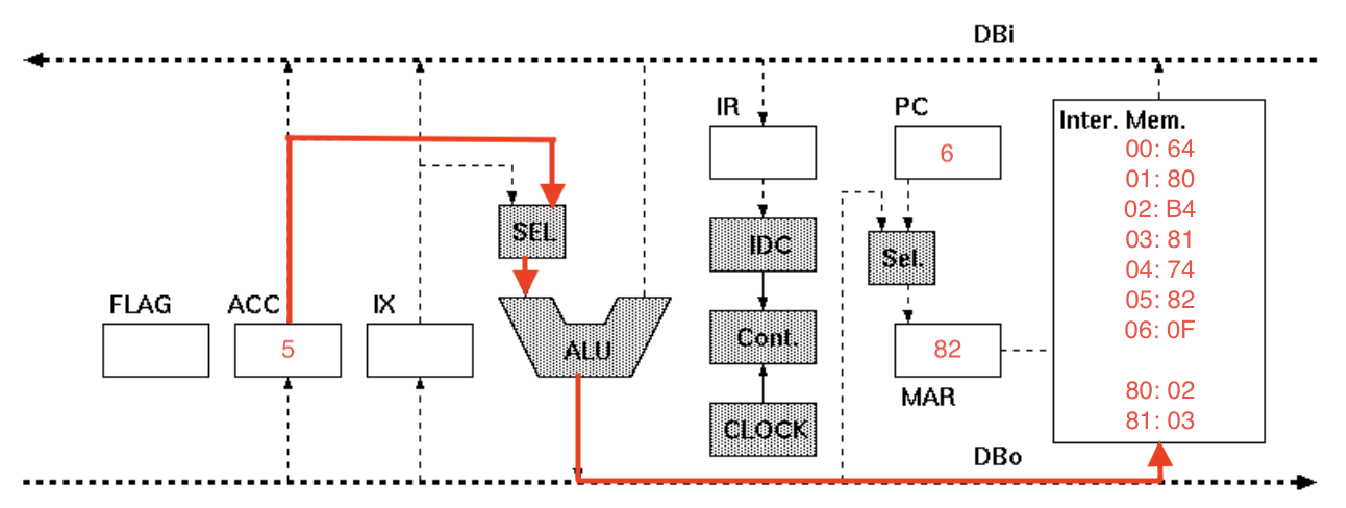
\includegraphics[scale=0.7]{img/st4.eps}% 図を貼り込む
            \vspace{-2mm}
            \subcaption{ST ACC, [ANS] P4時の値}
            \label{img:st4}
    \end{center}
    \caption{ST ACC時の各レジスタの値}
    \label{st}
\end{figure}

\clearpage

最後に,HLT命令について記述する.
\begin{description}
    \item[P0] PCの内容"06"をMARに転送する. \\ PCが示している06番地の命令を読み出すために,MARにPCの値を転送する.MARの内容は"06"となり,PCの値はインクリメントされる.
    \vspace{2mm}
    \item[P1] 命令内容の読み出しが行われる. \\ MARの内容で指定された06番地の内容(0F)が入力バスDBiを通り命令レジスタIRへ転送される.
    \vspace{2mm}
    \item[P2] 命令でコータIDCでIRの内容が解読される. \\ "00001- - -"のため,プログラムが停止する.
\end{description}



\subsection{各FLAGがどのような場合に変化するか}
\label{sec:flag}
本節では,表~\ref{table:add},表~\ref{table:adc}を用いて,各FLAGがどのような場合に変化するかを考察する.

まずはじめに,最終的なフラグレジスタの値は16進数で表記されているので,これらを2進数表記のなおす.
すると,ADD命令を用いた時の値はそれぞれ,$(0000 0000)_2$,$(0000 0110)_2$,$(0000 0010)_2$,$(0000 0010)_2$,$(0000 0100)_2$となる.
次に図~\ref{img:flag}のフラグレジスタを参考に値を比較すると,ADD命令を用いた時は式(2)ではフラグなし,式(3)では桁あふれフラグと負フラグ,式(4),(5)では負フラグ,式(6)では桁あふれフラグが立っている.
同様にADC命令を用いた時は式(3)では桁あふれフラグと負フラグ,式(4)では負フラグ,式(5)では桁あがりフラグと負フラグ,式(6)では桁あがりフラグと桁あふれフラグが立っている.
これらを踏まえて,各フラグがどのような場合に変化するかを考察する.

\subsubsection{桁あがりフラグについて}
これは,計算結果の桁数が増えた時に立つフラグであると考えられる.
式(5)において,$(-128)_{10}$というのは$(10000000)_2$であるから,計算結果が7桁から8桁に変化していることをフラグで知らせている.
また,ADD命令は使用せず,ADC命令が使用するフラグであると考察できる.

\subsubsection{桁あふれフラグについて}
これは,二進数8桁(16進数1桁)で表現しきれない値となった時に立つフラグであると考える.
式(3)において,実際の答えは128であるのに対して,計算結果は$(80)_h$であり,$(-128)_{10}$である.
繰り上がったものが補数と認識され,このような結果になったと考えられる.

\subsubsection{負フラグについて}
これは,計算結果が負の値の時に立つフラグであると考える.
補数を使用するため,その後の処理に問題が起きないよう,フラグを立てることで解決している.

\subsubsection{ゼロフラグについて}
今回の実験ではこのフラグが立つことはなかったが,これは,計算結果が0になった時に立つフラグであると予想できる.

\begin{figure}[htbp]
    \begin{center}
    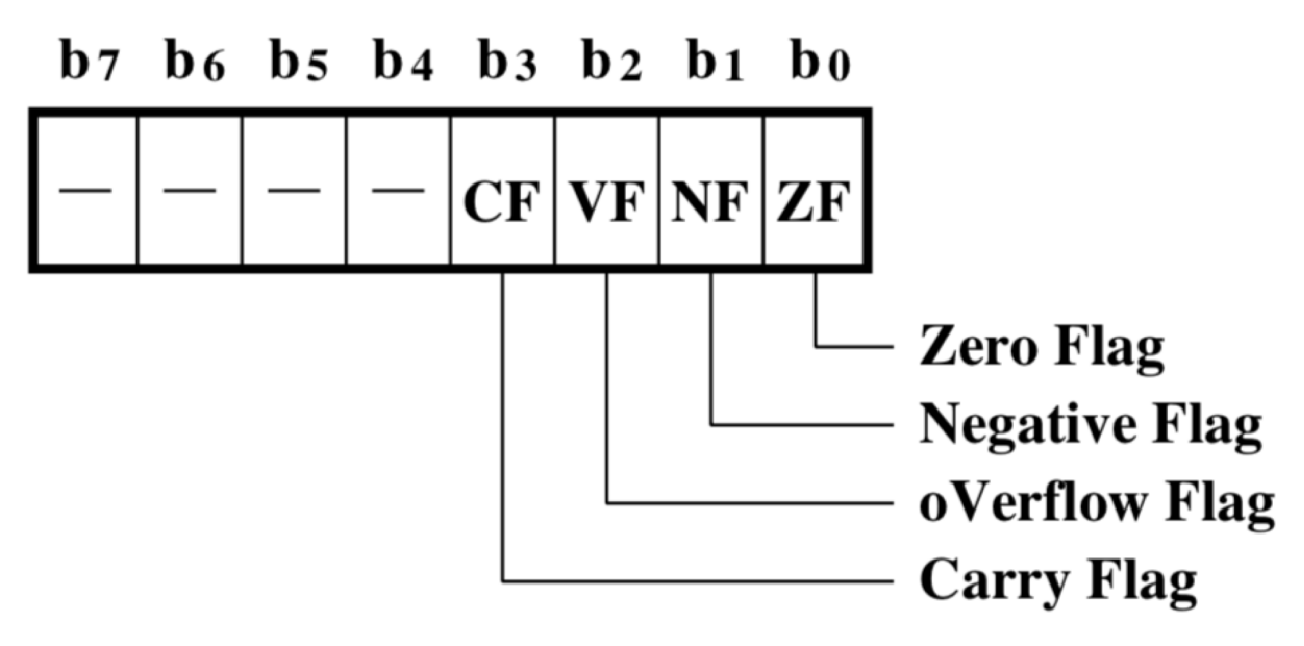
\includegraphics[scale=0.4]{img/flag.eps}% 図を貼り込む
    \end{center}
    \vspace{-8mm}
    \caption{フラグレジスタ}
    \label{img:flag}
\end{figure}

\subsection{ADDとADCの違い}
本節では,~\ref{sec:flag}節を用いてADD命令とADC命令の違いについて考察する.
ADD命令では桁あがりフラグを使用していなかったのに対し,ADC命令では桁あがりフラグを使用している.
つまり,ADD命令は半加算機のような動作をし,ADC命令は全加算機のような動きをすると考えられる.

\section{Problem 3.2 乗算プログラムの作成 }
\subsection{実験課題(方法)}
この課題では,フローチャートや,アセンブリ言語を用いたプログラムが与えられていない.
そのため,自分で乗算プログラムを作成する.
他人のプログラムと比較し,考察を行う.
\subsection{フローチャート・プログラムリスト}
図~\ref{img:flow}は作成したフローチャート図である.
また,ソースコード~\ref{program}に,本課題にて作成したプログラムリストを記述する.
なお,式を与えない状態でのフェーズ数は56となった.

なお,被乗数の1桁目をA,2桁目をBとし,乗数の1桁目をC,2桁目をD,答えの1桁目をE,2桁目をFとする.
\subsubsection{プログラムの説明}
このプログラムは以下の3つのフェーズに別れている.
\begin{enumerate}
    \item EにAの値をC回繰り返し足す
    \item FにBの値をC回繰り返し足す
    \item FにAの値をD回繰り返し足す
\end{enumerate}
本で,$B\times D$の計算がなされていないという点については,
与えられた問題の前提として,「答えは3桁にならない」という条件がある.
そのため,$B\times D$の計算は行っていない.

まず初めに,EとFを0で初期化する.
初期化を行ったら,次のフェーズに移行する.

1. このフェーズでは,EにAの値をC回繰り返し足すフェーズである.
\begin{enumerate}
    \item Cが0かを確認し,0でなければEにAの値を足す.0であればこのフェーズを終了する.
    \item 繰り上がりが起きていれば,Fの値をインクリメントする.
    \item Cの値をデクリメントし,1番に戻る.
\end{enumerate}

2. このフェーズでは,FにBの値をC回繰り返し足す.
なお,Bが0であった場合は0をB回足すことになり,非効率である.
そのため,Bが0であった場合は次のフェーズに移行する.
また,「答えは3桁にならない」という条件から,繰り上がりの処理は行っていない.
\begin{enumerate}
    \item Cが0かを確認し,0でなければFにBの値を足す.0であればこのフェーズを終了する.
    \item Cの値をデクリメントし,1番に戻る.
\end{enumerate}

3. このフェーズでは,FにAの値をD回繰り返し足す.
\begin{enumerate}
    \item Dが0かを確認し,0でなければFにAの値を足す.0であればこのフェーズを終了する.
    \item Dの値をデクリメントし,1番に戻る.
\end{enumerate}

\begin{figure}[H]
    \begin{center}
    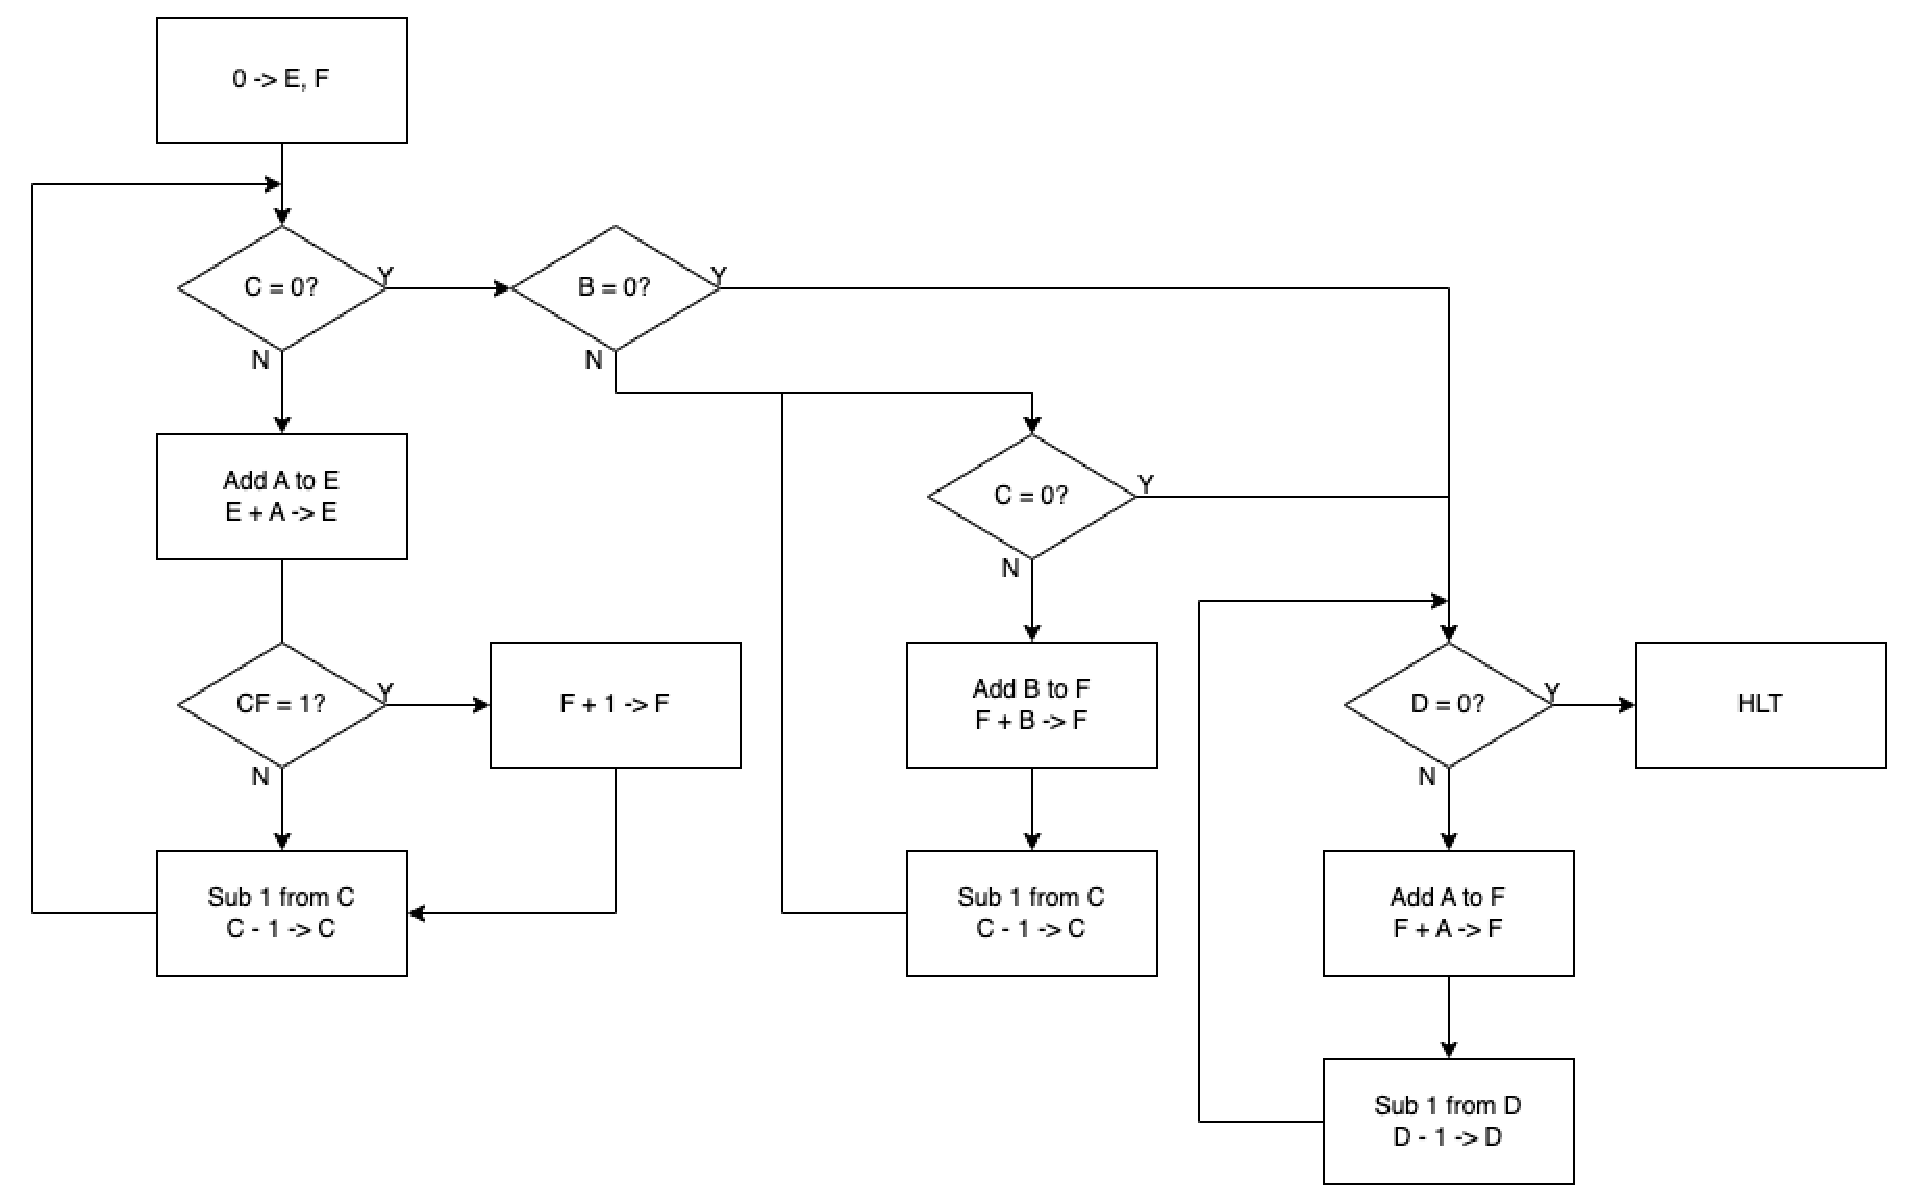
\includegraphics[scale=0.5]{img/flow.eps}% 図を貼り込む
    \end{center}
    \vspace{-3mm}
    \caption{乗算プログラムのフローチャート}
    \label{img:flow}
\end{figure}

\begin{lstlisting}[caption=乗算を行うプログラムリスト, label=program]
    80 :                   A:      EQU             80H
    81 :                   B:      EQU             81H
    82 :                   C:      EQU             82H
    83 :                   D:      EQU             83H
    84 :                   E:      EQU             84H
    85 :                   F:      EQU             85H
    00 :   62 00                   LD      ACC,    0
    02 :   74 84                   ST      ACC,    [E]
    04 :   74 85                   ST      ACC,    [F]
    06 :                   TOFIRST:                        
    06 :   6C 82                   LD      IX,     [C]
    08 :   AA 00                   SUB     IX,     0
    0A :   39 23                   BZ              TOSECOND
    0C :   30 0E                   BA              LOOP1
    0E :                   LOOP1:                  
    0E :   20                      RCF             
    0F :   64 84                   LD      ACC,    [E]
    11 :   94 80                   ADC     ACC,    [A]
    13 :   74 84                   ST      ACC,    [E]
    15 :   35 1D                   BNC             PASS1
    17 :   64 85                   LD      ACC,    [F]
    19 :   B2 01                   ADD     ACC,    1
    1B :   74 85                   ST      ACC,    [F]
    1D :                   PASS1:                  
    1D :   AA 01                   SUB     IX,     1
    1F :   39 23                   BZ              TOSECOND
    21 :   30 0E                   BA              LOOP1
    23 :                   TOSECOND:                       
    23 :   64 81                   LD      ACC,    [B]
    25 :   F2 00                   CMP     ACC,    0
    27 :   39 3E                   BZ              TOTHERD
    29 :   6C 82                   LD      IX,     [C]
    2B :   AA 00                   SUB     IX,     0
    2D :   39 3E                   BZ              TOTHERD
    2F :   30 31                   BA              LOOP2
    31 :                   LOOP2:                  
    31 :   20                      RCF             
    32 :   64 85                   LD      ACC,    [F]
    34 :   B4 81                   ADD     ACC,    [B]
    36 :   74 85                   ST      ACC,    [F]
    38 :   AA 01                   SUB     IX,     1
    3A :   39 3E                   BZ              TOTHERD
    3C :   30 31                   BA              LOOP2
    3E :                   TOTHERD:                        
    3E :   6C 83                   LD      IX,     [D]
    40 :   AA 00                   SUB     IX,     0
    42 :   39 53                   BZ              EXIT
    44 :   30 46                   BA              LOOP3
    46 :                   LOOP3:                  
    46 :   20                      RCF             
    47 :   64 85                   LD      ACC,    [F]
    49 :   B4 80                   ADD     ACC,    [A]
    4B :   74 85                   ST      ACC,    [F]
    4D :   AA 01                   SUB     IX,     1
    4F :   39 53                   BZ              EXIT
    51 :   30 46                   BA              LOOP3
    53 :                   EXIT:                   
    53 :   0F                      HLT             
                                   END
\end{lstlisting}

\subsection{他人のプログラムとの比較}
図~\ref{img:flow}を元に作成したプログラムのByte数は88Byteとなった.
表~\ref{table:fast}は実行時間計測用の式である.
また,表~\ref{table:time}は各プログラムのByte数,実行時間をまとめた表である.
なお,実行時間は四捨五入を行っている.

これらの表からわかることとして,3人の間にプログラムサイズの大きな差はないことがわかる.
はじめに,\textcircled{\scriptsize A}式よりも\textcircled{\scriptsize B}式の実行時間が大きい結果となった.
考察として,\textcircled{\scriptsize A}式では,それぞれ$(25)_{h}$回の計算を繰り返しているのに対して,
\textcircled{\scriptsize B}式では$(AB)_{h}$回,$(3)_{h}$回の計算を繰り返している.
つまり,繰り返しの量が実行時間に影響を及ぼしていると考えることができる.
このプログラムの改善案として,被乗数と乗数の値を比較し,被乗数と乗数を入れ替える操作を行うことで更なる実行時間の短縮が見込める.

結城君のプログラムでは上記の改善案を取り入れて,作成していた.この操作によって\textcircled{\scriptsize A}式,\textcircled{\scriptsize B}式ともに21秒という結果になったのだろう.
また,末本君のプログラムでは,シフト演算を用いて乗算を行っていた.シフト演算を用いた乗算では,乗数のビット数だけ比較・シフト演算を行うので,足し算の繰り返しよりも実行時間が短い結果となった.


\begin{table}[H]
    \centering
    \caption{プログラム計測用の乗算}
    \label{table:fast}
    \begin{minipage}[b]{0.49\columnwidth}
        \centering
        \begin{tabular}{cc}
            \textcircled{\scriptsize A}& 03AB \\
            $\times$ & 0025 \\
            \hline
            & 87B7
        \end{tabular}
    \end{minipage}
    %
    \begin{minipage}[b]{0.49\columnwidth}
        \centering
        \begin{tabular}{cc}
            \textcircled{\scriptsize B}& 0025 \\
            $\times$ & 03AB \\
            \hline
            & 87B7
        \end{tabular}
    \end{minipage}
\end{table}

\begin{table}[H]
    \centering
    \caption{各プログラムの実行時間}
    \label{table:time}
    \begin{tabular}{|c|c|c|c|}
        名前 & 使用Byte数 & \textcircled{\scriptsize A}式の実行時間 & \textcircled{\scriptsize B}式の実行時間 \\
        高砂 & 88Byte & 28秒 & 63秒 \\
        結城 & 74Byte & 21秒 & 21秒 \\
        末本 & 89Byte & 8秒 & 12秒
    \end{tabular}
\end{table}

    

% \begin{table}[H]
%     \centering
%     \caption{プログラム確認用の乗算}
%     \label{table:times}
%     \begin{minipage}[b]{0.24\columnwidth}
%         \centering
%         \begin{tabular}{cc}
%             \textcircled{\scriptsize 1}& 0028 \\
%             $\times$ & 04CD \\
%             \hline
%             & C008
%         \end{tabular}
%     \end{minipage}
%     %
%     \begin{minipage}[b]{0.24\columnwidth}
%         \centering
%         \begin{tabular}{cc}
%             \textcircled{\scriptsize 2}& 00FC \\
%             $\times$ & 00AE \\
%             \hline
%             & AB48
%         \end{tabular}
%     \end{minipage}
% %
%     \begin{minipage}[b]{0.24\columnwidth}
%         \centering
%         \begin{tabular}{cc}
%             \textcircled{\scriptsize 3}& 03AB \\
%             $\times$ & 0025 \\
%             \hline
%             & 87B7
%         \end{tabular}
%     \end{minipage}
% %
%     \begin{minipage}[b]{0.24\columnwidth}
%         \centering
%         \begin{tabular}{cc}
%             \textcircled{\scriptsize 4}& 132D \\
%             $\times$ & 000B \\
%             \hline
%             & D2EF
%         \end{tabular}
%     \end{minipage}
% \end{table}

% \begin{enumerate}
%     \item 1分16秒
%     \item 1分24秒
%     \item 28秒
%     \item 8秒
% \end{enumerate}

\subsection{理論値の計算・実測値との比較}
本説では,実行時間の計測に使用した2式をもとに実行時間の理論値・実測値との比較を行う.
今回の実験では,クロックを100Hzに設定し実験を行った.
また,1クロックで1フェーズ進むことから,1フェーズにかかる実行時間の理論値は10ミリ秒であることが考えられる.
よって,実行時間の理論値を算出するためには,計算時の総フェーズ数を求めることで理論値が求められると考える.
総フェーズ数を求めるため,プログラム\ref{program}を用いて算出する.
なお,\textcircled{\scriptsize A}式の実行時間の実測値は28秒,\textcircled{\scriptsize B}式の実行時間の実測値は63秒である.

\textcircled{\scriptsize A}式では,
まず,04番地にて,ACCの値を[F]にSTOREするまで$14$フェーズ使用している.
次に,06番地にて,[C]の値をIXに転送,IXの減算,比較しLOOP1に行くまでで,$17$フェーズ使用している.
LOOP1では,繰り上がりをしない場合は34フェーズ,繰り上がりをする場合は48フェーズ使用する.
今回の式は,37ループ中,24回繰り上がりを行うが,最後の足し算のみ分岐にて,TOSECONDに行くので,34フェーズではなく,30フェーズとなる.
よって,$(34\times12) + (48\times24) + 30 = 1,590$フェーズ使用している.
次に,23番地にて,[B]の値をACCに転送してから,LOOP2に行くまでで,$30$フェーズ使用する.
LOOP2では,一回繰り返すのに,30フェーズ使用し,繰り上がりを考慮しないが,ここでも,最後の足し算のみ分岐にて,TOTHERDに行くので,30フェーズではなく,26フェーズとなる.
よって,$30\times36 + 26 = 1,106$フェーズ使用している.
次に,3E番地にて,[D]の値をIXに転送してから,HLT命令に行くまでで,$13$フェーズ使用し,HLTで$3$フェーズ使用し,プログラムが終了する.
よって,\textcircled{\scriptsize A}式を計算する際の総フェーズ数は2,773フェーズ,実行時間の理論値は27.73秒となる.
実測値は28秒であったので,概ね良い結果となった.

\textcircled{\scriptsize B}式でも同様に考えると,
LOOP1までに$31$フェーズ使用し,
LOOP1では,171ループ中,24回繰り上がりを行うので,$(34\times146) + (48\times24) + 30 = 6,146$フェーズ,
LOOP3までに$30$フェーズ使用し,
LOOP3では,$30\times2 + 26 = 86$フェーズ,
HLTに$3$フェーズ使用し,プログラムが終了する.
よって,\textcircled{\scriptsize B}式を計算する際の総フェーズ数は6,296フェーズ,実行時間の理論値は62.96秒となる.
実測値は63秒であったので,こちらも同様に良い結果となった.


\end{document}
